\section{Main-Challenge Task Inventory}
\label{app:tasks}

\begin{table}[h]
\centering
\scriptsize
\caption{Main \geneexam{} challenge: 42 task types across 4 capability dimensions, totaling 1,029 instances. Calibration/local-matching diagnostics are retained in the code release but excluded from the paper leaderboard.}
\label{tab:all_tasks}
\begin{tabular}{@{}p{1.15cm}p{1.2cm}p{5.35cm}r@{}}
\toprule
\textbf{Axis} & \textbf{ID} & \textbf{Task Type} & \textbf{N} \\
\midrule
\multirow{5}{*}{T1} & T1-01 & Contribution Role & 30 \\
& T1-02 & Genome-Field Type & 25 \\
& T1-03 & Driver-Passenger Roles & 20 \\
& T1-04 & Lineage Position & 25 \\
& T1-05 & Cross-Lineage Bridge & 25 \\
\midrule
\multirow{12}{*}{T2} & T2-01 & Five-Genome Lineage Reconstruction & 25 \\
& T2-02 & Six-Genome Lineage Reconstruction & 25 \\
& T2-03 & Seven-Genome Lineage Reconstruction & 25 \\
& T2-04 & Lineage Grouping (8) & 25 \\
& T2-05 & Medium Lineage Grouping (8) & 25 \\
& T2-06 & Three-Lineage Grouping (9) & 25 \\
& T2-07 & Limitation-Delta Match & 25 \\
& T2-08 & Mixed Limitation-Delta Match & 25 \\
& T2-09 & Chained Limitation-Delta Match & 25 \\
& T2-10 & Two-Paper Genome-Field Assignment & 29 \\
& T2-11 & Three-Paper Genome-Field Assignment & 29 \\
& T2-12 & Genome Alignment & 30 \\
\midrule
\multirow{17}{*}{T3} & T3-01 & Single-Step Dynamics & 25 \\
& T3-02 & Genome-Field Fate & 25 \\
& T3-03 & Driver Dynamics & 25 \\
& T3-04 & Shown Genome-Field Fate & 22 \\
& T3-05 & Driver-Fate Summary & 23 \\
& T3-06 & Mechanism-Only Dynamics & 25 \\
& T3-07 & Blind Genome-Field Fate & 25 \\
& T3-08 & Unlabeled Driver Inference & 24 \\
& T3-09 & Relation Classification & 21 \\
& T3-10 & Directional Genome Choice & 25 \\
& T3-11 & Evolutionary Tempo & 30 \\
& T3-12 & Evolutionary Pattern & 25 \\
& T3-13 & Hidden Genome Fate & 24 \\
& T3-14 & Hybrid Provenance & 25 \\
& T3-15 & Multi-Hop Genome Tracking & 20 \\
& T3-16 & Dynamics Boundary & 25 \\
& T3-17 & Multi-Citation Relation & 20 \\
\midrule
\multirow{8}{*}{T4} & T4-01 & Genome Consistency Check & 25 \\
& T4-02 & Domain Intruder Detection & 25 \\
& T4-03 & Local Lineage Repair & 25 \\
& T4-04 & Next-Hop Prediction & 24 \\
& T4-05 & Parent-Genome Identification & 25 \\
& T4-06 & Missing-Link Recovery & 18 \\
& T4-07 & Genome-Bridge Validation & 20 \\
& T4-08 & Citation Consistency & 20 \\
\bottomrule
\end{tabular}
\end{table}

\begin{table}[h]
\centering
\scriptsize
\caption{Active \genearena{} task inventory for the main run: 30 tasks balanced across 10 scientific domains.}
\label{tab:traces}
\begin{tabular}{p{2.6cm}p{8.1cm}c}
\toprule
\textbf{Domain} & \textbf{Task Type} & \textbf{Count} \\
\midrule
Computer Science & AgentFramework, LLMReasoning, NativeMultimodal & 3 \\
Biology & ProteinDesign, SingleCellFoundation, SpatialTranscriptomics & 3 \\
Chemistry & DrugDiscovery, MolecularGeneration, Retrosynthesis & 3 \\
Climate & AtmosphericChemistry, ClimateSimulation, WeatherForecasting & 3 \\
Energy & BatteryOptimization, PerovskiteSolarCell, SmartGridOptimization & 3 \\
Materials & BatteryElectrolyte, Catalysis, Discovery & 3 \\
Mathematics & AIforCombinatorics, AutomatedTheoremProving, MathReasoning & 3 \\
Medicine & DrugRepurposing, MedicalFoundationModels, MedicalImageAnalysis & 3 \\
Neuroscience & BrainComputer, Connectomics, VisualCortex & 3 \\
Physics & FusionPlasmaControl, NeuralNetworkPotentials, QuantumErrorCorrection & 3 \\
\midrule
\textbf{Total} & & \textbf{30 active} \\
\bottomrule
\end{tabular}
\end{table}

\section{\gene{} Examples}
\label{app:examples}

\subsection{\geneexam{}}
\label{app:ex_exam}

We present one representative example per capability dimension (T1--T4), showing the full question, choices, and gold answer.

%% ───────────────────────────────────────────────
\begin{tcolorbox}[
    breakable,
    title={Example of T1 · Genome Abstraction (T1-01: Contribution Role)},
    colback=LighterGray,
    colframe=DeepPurple,
    colbacktitle=DeepPurple,
    coltitle=White,
]
\textbf{\textcolor{CaseOrange}{Question.}} Given an anonymized genome extracted from a paper, classify its contribution type.
Options: \texttt{method}, \texttt{dataset}, \texttt{analysis}, \texttt{system}, \texttt{theory}.

\medskip
\textit{Claim}: ``A probabilistic model that accounts for repertoire-specific maturation age can reliably recover the true landscape and length statistics of antibody somatic indels from sequencing data.''\\
\textit{Delta}: ``Provides a dedicated probabilistic method for unbiased learning of antibody indel statistics, compared with prior work relying on biased annotation-based indel calls.''\\
\textit{Observation}: ``Applied to large human heavy-chain datasets, the model finds distinct insertion/deletion hotspots and shows indel lengths are approximately geometrically distributed.''

\medskip
\textbf{\textcolor{CaseBlue}{Answer:}} \texttt{method} \quad
\textit{(The paper introduces a new probabilistic model — a clear methodological contribution.)}
\end{tcolorbox}

\bigskip

%% ───────────────────────────────────────────────
\begin{tcolorbox}[
    breakable,
    title={Example of T2 · Inheritance Tracing (T2-04: Lineage Grouping)},
    colback=LighterGray,
    colframe=DeepPurple,
    colbacktitle=DeepPurple,
    coltitle=White,
]
\textbf{\textcolor{CaseOrange}{Question.}} Eight \genome{} objects are presented in shuffled order. Partition them into exactly two lineage groups of four objects each, ordered from earliest to latest.

\smallskip
\textbf{P}: \textit{``Directly optimize a neural architecture policy using RL to assign layer-wise operations.''}\\
\textbf{Q}: \textit{``NIN replaces fully-connected layers with global average pooling and $1{\times}1$ conv to deepen non-linearity.''}\\
\textbf{R}: \textit{``DARTS relaxes the discrete architecture search space into a continuous one via differentiable mixed-operation weights.''}\\
\textbf{S}: \textit{``Inception-v3 factorizes large convolutions into asymmetric sequences to reduce parameters.''}\\
\textbf{T}: \textit{``EfficientNet jointly scales width, depth, and resolution via compound coefficients.''}\\
\textbf{U}: \textit{``ENAS shares weights across child networks to reduce NAS search cost by orders of magnitude.''}\\
\textbf{V}: \textit{``GoogLeNet stacks Inception modules to achieve high accuracy at low parameter cost.''}\\
\textbf{W}: \textit{``MnasNet uses RL-based NAS with mobile hardware latency as a proxy reward.''}

\medskip
\textbf{\textcolor{CaseBlue}{Answer:}}
\begin{quote}\small
\textbf{Group 1 (NAS-RL lineage):} P $\to$ U $\to$ R $\to$ W\\
\textbf{Group 2 (Inception lineage):} Q $\to$ V $\to$ S $\to$ T
\end{quote}
\textit{Why}: Group 1 shares a lineage of learning architectural decisions (RL search $\to$ weight sharing $\to$ differentiable relaxation $\to$ mobile NAS); Group 2 shares the Inception niche of efficient multi-scale feature extraction.
\end{tcolorbox}

\bigskip

%% ───────────────────────────────────────────────
\begin{tcolorbox}[
    breakable,
    title={Example of T3 · Evolutionary Dynamics (T3-01: Single-Step Dynamics)},
    colback=LighterGray,
    colframe=DeepPurple,
    colbacktitle=DeepPurple,
    coltitle=White,
]
\textbf{\textcolor{CaseOrange}{Question.}} Given the Niche and Mechanism of predecessor A and successor B, identify the primary evolutionary dynamic.

\smallskip
\textbf{Predecessor A:}\\
\textit{Niche}: ``Understanding and improving robustness of neural network classifiers to small, intentionally constructed input perturbations that cause misclassification.''\\
\textit{Mechanism}: ``FGSM linearizes the loss at the input point, computes the gradient w.r.t.\ the input, takes its element-wise sign, and adds a small $\epsilon$-perturbation under $\ell_\infty$ constraint to generate an approximate worst-case sample.''

\smallskip
\textbf{Successor B:}\\
\textit{Niche}: ``Understanding \emph{why} deep neural network classifiers remain vulnerable to adversarial perturbations despite strong generalization on natural inputs.''\\
\textit{Mechanism}: ``Uses first-order linear analysis to explain adversarial examples, modeling classifiers as locally linear in high-dimensional input space: a perturbation chosen along the input gradient accumulates across many dimensions to significantly alter class scores.''

\medskip
\textbf{\textcolor{CaseOrange}{Choices:}}
\begin{quote}\small
A.\ Mutation \quad B.\ Adaptive Radiation \quad C.\ Hybridization \quad D.\ Speciation \quad E.\ Niche Competition
\end{quote}

\textbf{\textcolor{CaseBlue}{Answer: A.\ Mutation}}\\
\textit{Why}: B inherits and refines A's first-order gradient-sign mechanism, while narrowing to a theoretical niche (explaining vulnerability) — a local modification, not a structural departure.
\end{tcolorbox}

\bigskip

%% ───────────────────────────────────────────────
\begin{tcolorbox}[
    breakable,
    title={Example of T4 · Structural Integrity (T4-06: Missing-Link Recovery)},
    colback=LighterGray,
    colframe=DeepPurple,
    colbacktitle=DeepPurple,
    coltitle=White,
]
\textbf{\textcolor{CaseOrange}{Question.}} Paper A and Paper C are given; identify the missing bridge paper B from four candidates.

\smallskip
\textbf{Paper A}: ``Balance control for legged robots using ZMP-based model predictive control; focuses on stability under static and slow dynamic gaits.''

\textbf{Paper C}: ``Sim-to-real RL for agile locomotion; trains a neural network policy end-to-end in simulation and deploys on hardware using domain randomization.''

\medskip
\textbf{\textcolor{CaseOrange}{Candidates:}}\\
\textbf{X}: ``A dataset of human gait trajectories for imitation learning.''\\
\textbf{Y}: ``A periodic gait stabilization framework that decouples cycle generation from balance correction, enabling classical controllers to handle dynamic terrain.''\\
\textbf{Z}: ``A transformer-based language model for robot task planning.''\\
\textbf{W}: ``A convolutional terrain classifier for foothold selection.''

\medskip
\textbf{\textcolor{CaseBlue}{Answer: Y}}\\
\textit{Why}: Y bridges A's model-predictive stability focus and C's RL-based locomotion by introducing a periodic gait framework — a structural predecessor that made dynamic, policy-compatible gait generation feasible before the RL era.
\end{tcolorbox}

\subsection{\genearena{}}
\label{app:ex_arena}

%% ───────────────────────────────────────────────
\begin{tcolorbox}[
    breakable,
    title={Example of \genearena{} · Pairwise Idea Battle (Physics / Fusion Plasma Control)},
    colback=LighterGray,
    colframe=DeepPurple,
    colbacktitle=DeepPurple,
    coltitle=White,
]
\textbf{\textcolor{CaseOrange}{Question.}} Given a frontier research question and two anonymously generated ideas, judge which idea is stronger based on lineage grounding, meaningful variation, and selection value for future research. Options: \textbf{A}, \textbf{B}, or \textbf{Tie}.

\medskip
\textit{Frontier question}: Predict-first TCV and RL plasma-control studies show that data-driven control can learn device-specific dynamics, but ITER-scale deployment needs cross-device transfer, uncertainty-aware safety, and simulator-to-shot adaptation. What fusion-control foundation model would combine differentiable plasma simulators, multi-tokamak logs, and constrained RL to produce robust ramp-up, sustainment, and ramp-down policies across machines?

\medskip
\textbf{Idea A — Uncertainty-Aware Tokamak Control Foundation Model.}
Pretrain a transformer/state-space latent dynamics model on multi-tokamak time-series data (DIII-D, TCV, JET, EAST, C-Mod, HL-3 and TORAX rollouts), coupled to differentiable TORAX physics with learned residuals. Train constrained model-based RL policies with Bayesian uncertainty estimates and runtime safety shields (tearing, shape, density, disruption budgets). Before deployment, calibrate via a small number of predict-first target-machine shots updating Bayesian residuals — without retraining the full model.

\medskip
\textbf{Idea B — FusionFoundationRL: Cross-Tokamak Differentiable-Constrained Policy.}
Combine TORAX's differentiable physics engine with a neural state-space model (NSSM) into a hybrid dynamics foundation model trained on multi-tokamak logs. Device-specific parameters (geometry, coil limits) are encoded as context vectors. A constrained RL agent uses cross-machine tearing/disruption predictors as safety bounds, and TORAX's differentiability initializes the policy via gradient-based optimization. Unified ramp-up, sustainment, and ramp-down in a single policy, with simulator-to-shot fine-tuning for adaptation.

\medskip
\textit{Which idea better addresses the frontier? Consider: how well does each inherit and build on prior work, how meaningfully does it advance beyond it, and how much does it open new research directions?}
\end{tcolorbox}

\bigskip

%% ───────────────────────────────────────────────
\begin{tcolorbox}[
    breakable,
    title={Example of \genearena{} · Battle with Judge Result (Biology / Protein Design)},
    colback=LighterGray,
    colframe=DeepPurple,
    colbacktitle=DeepPurple,
    coltitle=White,
]
\textbf{\textcolor{CaseOrange}{Frontier question.}}
Design de novo protein binders against therapeutic targets where high in silico affinity does not reliably translate into selective, stable, functional activity in living cells.
What generative framework would close the loop between computational design and in vivo biological function?

\medskip
\textbf{Idea A — Cell-in-the-Loop Multi-Objective Protein Binder Design.}
Couple structure-based binder generation (diffusion/flow-matching conditioned on target epitope, off-target panels, and stability constraints) with a learned multi-fidelity fitness model. Candidate designs are scored by a differentiable surrogate ensemble covering binding affinity, target selectivity, folding stability, expression, and cell-based efficacy. A causal latent variable model separates true target engagement from confounders (expression level, trafficking, toxicity). The surrogate is updated iteratively via active learning from barcoded pooled yeast/mammalian display and cellular reporter assays, converting protein binder design into a self-improving closed-loop system optimized for experimentally meaningful activity.

\medskip
\textbf{Idea B — Multi-Constraint Latent Diffusion for In-Vivo-Aware Protein Binder Design.}
Learn a unified latent representation from multi-modal data (structures, binding assays, biophysical stability, in vivo functional readouts) using a multi-modal VAE, then run a conditional diffusion model in this latent space guided by target structure embeddings and a learned biological constraint manifold. A differentiable in vivo efficacy surrogate provides gradient feedback during generation; selectivity is enforced by contrastive learning against off-target proteomes; stability is modeled via physics-informed neural networks. A Pareto-frontier multi-objective reward balances competing constraints, aiming to raise experimental validation rates from $\sim$5--10\% to $>$30\%.

\medskip
\textbf{\textcolor{CaseBlue}{Judge result: Idea A wins.}}\\
\textbf{\textcolor{CaseBlue}{Judge reason:}} \textit{``Idea A more cleanly extends the frontier lineage by preserving structure-first generative design while adding assay-grounded active learning and causal components that directly target the known in silico-to-function gap, with a more feasible validation plan. Idea B is ambitious but relies on weakly transferable in vivo surrogates and expensive mouse-model validation.''}
\end{tcolorbox}



\section{Evaluation Details}
\label{app:eval_logging}

All \geneexam{} runs write the decoding budget into the top-level JSON metadata as \texttt{max\_output\_tokens}. Per-instance logs also store input/output token counts when returned by the API, response length, extraction diagnostics, and an error class. Empty responses are therefore separated into API failures, missing-format outputs, and token-budget exhaustion rather than being silently counted as ordinary content errors.

This detail matters for reasoning-heavy deployments. In pilot GPT-5.5 runs, a 4,096-token completion cap sometimes produced empty visible answers while the API reported the full output budget as consumed. We therefore use a 16,384-token cap for GPT-5.5 main-challenge reruns and keep the cap in the released logs so that scores remain auditable across providers and reruns. The paper leaderboard reports the same exact-match metric for all models; token-budget metadata is used only for diagnosis and reproducibility, not for changing an instance score.


\section{Human Agreement}
We recruited 50 graduate annotators (master’s and doctoral students across
computer science, biology, physics, materials science, and other disciplines) to validate the benchmark
at three stages: \genomediff{} relation labels and role-type assignments during construction (disagreements adjudicated; ambiguous items excluded), \geneexam{} item difficulty through stratified
human solving to confirm low accuracy reflects compositional challenge rather than label noise, and
\genearena{} ELO battles where human judges reached 80\% agreement with the strongest model-judge panel on pairwise preference comparisons. PES scoring uses the same lineage packet format for model and human audit: judges see the frontier question, relevant \genome{} objects, \genomediff{} evidence, and population neighborhood before assigning H/V/S. This concordance supports scalable model-judge evaluation while confirming that scoring criteria are reproducible by trained domain experts.

\section{Additional \genearena{} Analysis}
\label{app:arena_analysis}

\subsection{Domain-Level PES}

This view checks whether lineage-grounded generation quality is uniform across scientific domains. Each cell averages Lineage-setting PES over the three active frontier tasks in that domain, so row-wise variation exposes domain-specific weaknesses that are hidden by a single overall PES.

\begin{figure}[h]
\centering
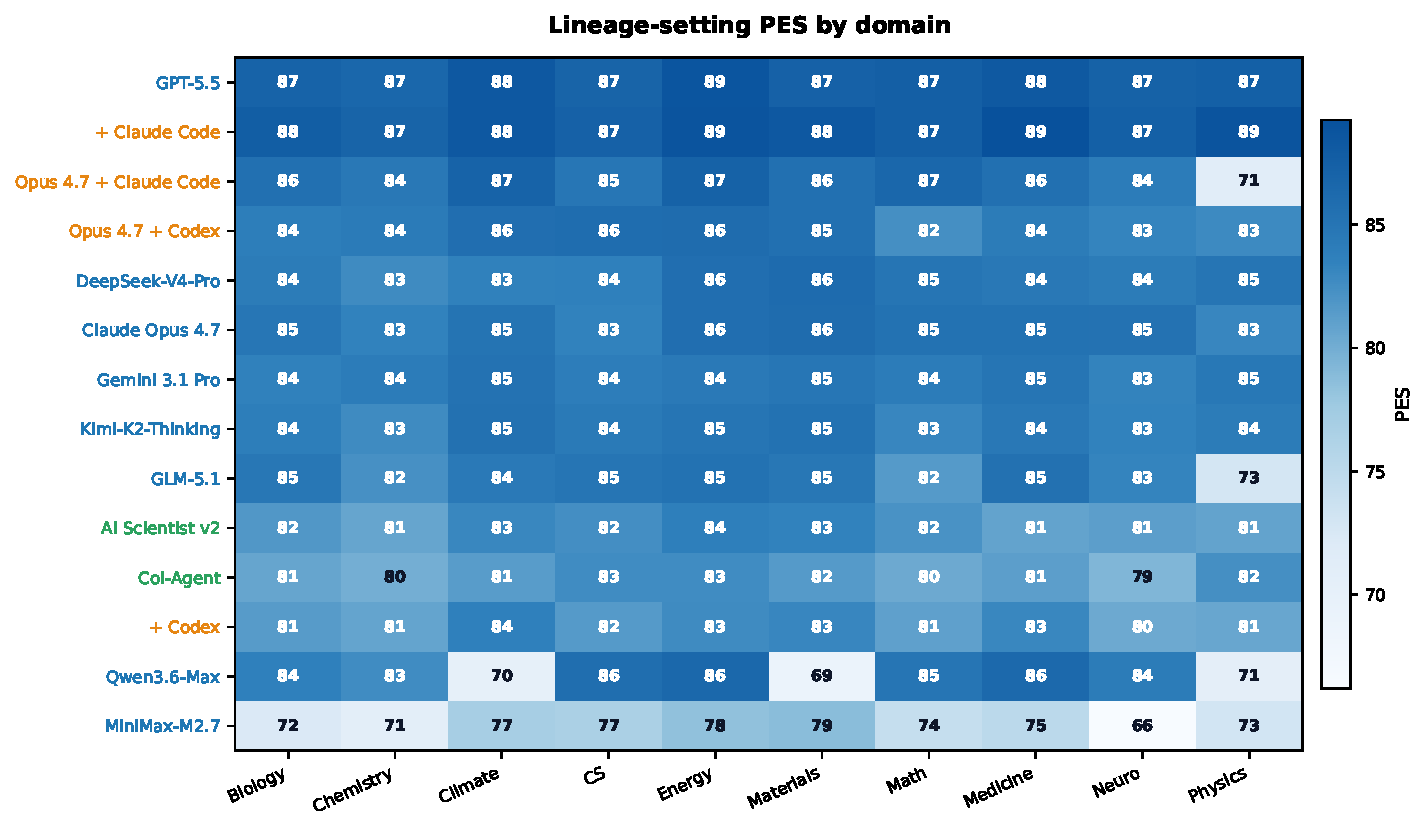
\includegraphics[width=\textwidth]{figures/pes_domain_heatmap.pdf}
\caption{\textbf{Domain-level PES snapshot.} Lineage-setting PES across 10 domains for the evaluated systems. Strong systems remain relatively uniform, while weaker systems show sharper domain-specific failures.}
\label{fig:pes_domain_app}
\end{figure}

\subsection{PES Decomposition and Information-Setting Breakdown}

This pair of heatmaps decomposes PES along two orthogonal axes. Panel~(a) separates the three rubric components---Heredity, Variation, Selection---to show whether high PES comes from coherent inheritance, meaningful novelty, or downstream viability; the recurring Variation-over-Heredity pattern is the main evidence for the plausibility--coherence gap discussed in the main text. Panel~(b) isolates what each information setting contributes: Question-only prompts test parametric ideation, Library adds unordered paper context, and Lineage adds ordered \genome{} objects plus \genomediff{} evidence; heterogeneous gains show that lineage evidence is useful only when a system can operationalize it.

\begin{figure}[h]
\centering
\begin{subfigure}[t]{0.48\textwidth}
\centering
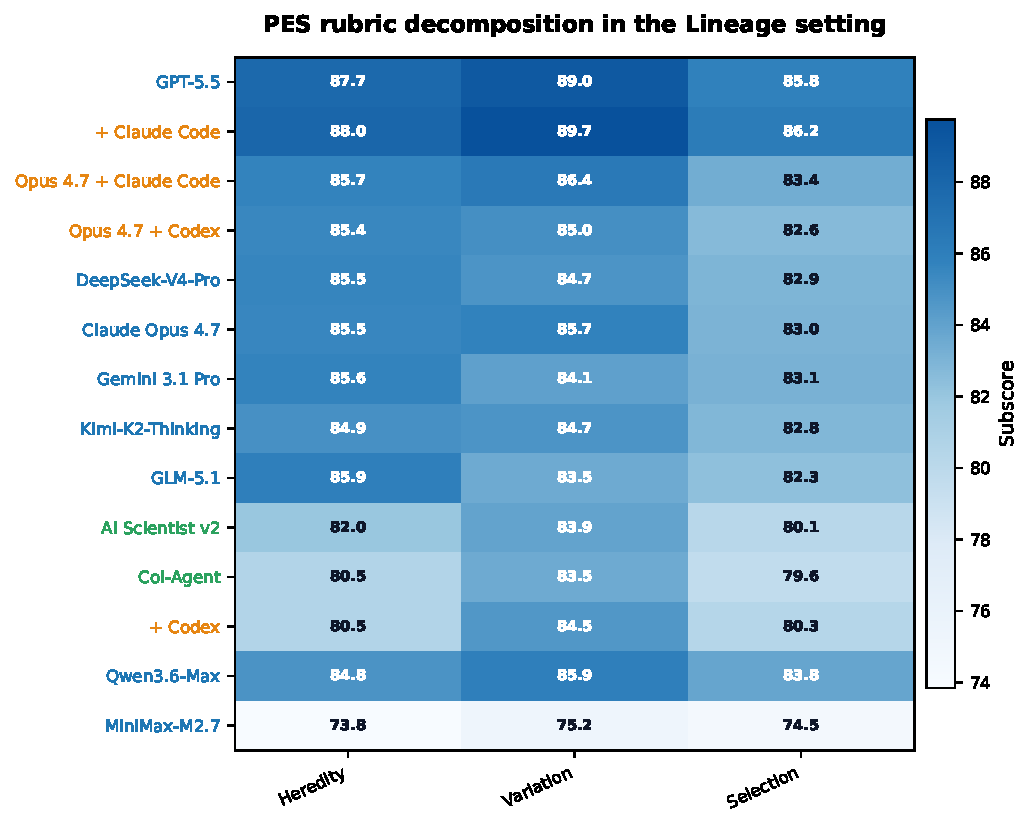
\includegraphics[width=\linewidth]{figures/pes_dimension_breakdown.pdf}
\caption{PES rubric decomposition (H / V / S).}
\end{subfigure}\hfill
\begin{subfigure}[t]{0.48\textwidth}
\centering
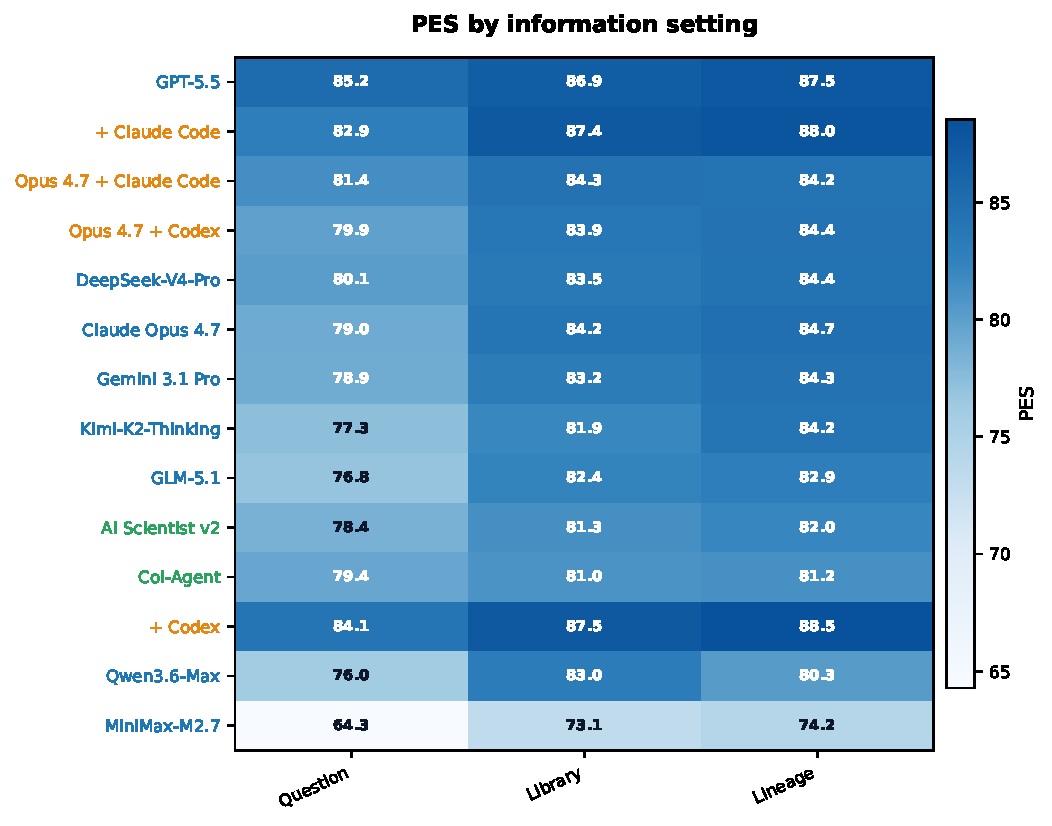
\includegraphics[width=\linewidth]{figures/pes_setting_breakdown.pdf}
\caption{PES by information setting (Question / Library / Lineage).}
\end{subfigure}
\caption{\textbf{PES decomposition and information-setting breakdown.} (a)~Heredity, Variation, and Selection sub-scores under the genome-centric scoring packet. Variation consistently exceeds Heredity across systems, confirming the plausibility--coherence gap identified in Finding~3. (b)~PES under Question, Library, and Lineage settings. Question$\to$Lineage gains are heterogeneous: GPT-5.5 moves only from 85.2 to 87.5, while weaker systems gain more from explicit lineage context.}
\label{fig:pes_dim_app}
\end{figure}

\subsection{Generated Dynamics Distribution}

This figure preserves the raw frequency view replaced by the main-text dynamics quality map. It shows that Question-only prompts produce a broader mix of evolutionary moves, while Library and Lineage prompts concentrate on Hybridization; by itself, however, this distribution cannot tell whether the recombination is genetically coherent.

\begin{figure}[h]
\centering
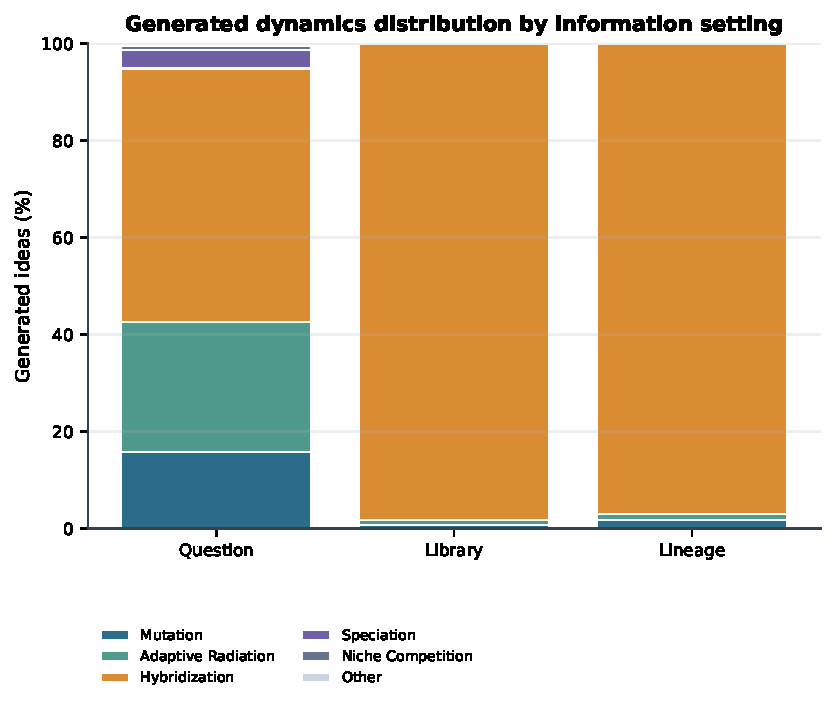
\includegraphics[width=0.58\textwidth]{figures/arena_dynamics_distribution.pdf}
\caption{\textbf{Generated dynamics distribution by information setting.} Stacked proportions of post-hoc dynamics labels for generated \genearena{} proposals. The main text replaces this pure frequency view with a quality map because the same dynamics label can have different Heredity and PES depending on whether lineage evidence is available.}
\label{fig:arena_dynamics_dist_app}
\end{figure}

\subsection{Per-System H/V/S Bar Chart}

This bar chart provides a ranking-oriented view of the same Lineage-setting H/V/S decomposition shown in the heatmap above. Systems are sorted by Lineage PES; the visual separation between Variation and Heredity bars confirms that the plausibility--coherence gap is systematic across all 14 participants.

\begin{figure}[h]
\centering
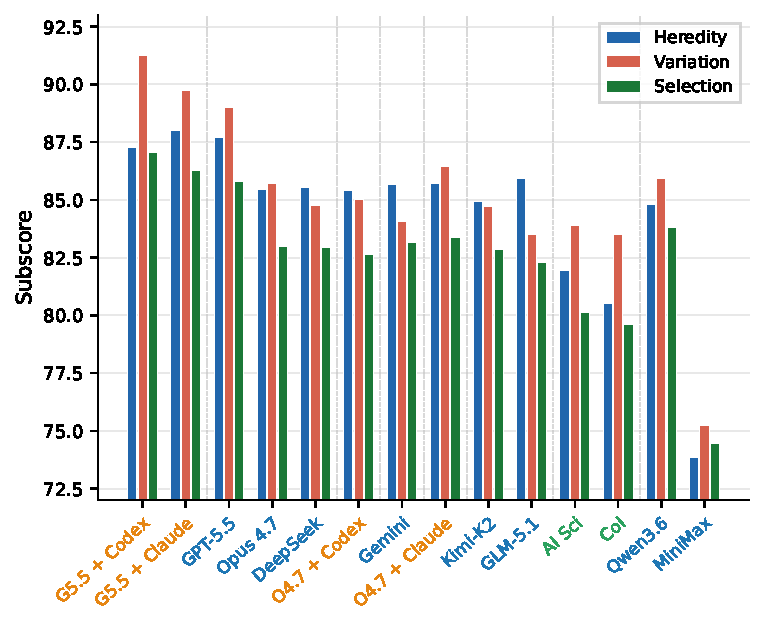
\includegraphics[width=0.58\textwidth]{figures/pes_dimension_breakdown_main.pdf}
\caption{\textbf{Per-system H/V/S bar chart.} Lineage-setting Heredity, Variation, and Selection for all evaluated systems, sorted by aggregate Lineage PES. Variation consistently exceeds Heredity, confirming the plausibility--coherence gap across the full participant set.}
\label{fig:pes_bars_app}
\end{figure}

\FloatBarrier

\section{Additional \geneexam{} Analysis}
\label{app:exam_analysis}

\subsection{\geneexam{} Main-Leaderboard Heatmap}

This heatmap reports the main leaderboard's exact accuracy across T1--T4. We keep it here as the detailed closed-form diagnostic view while the main text uses the more compact radar profile.

\begin{figure}[h]
\centering
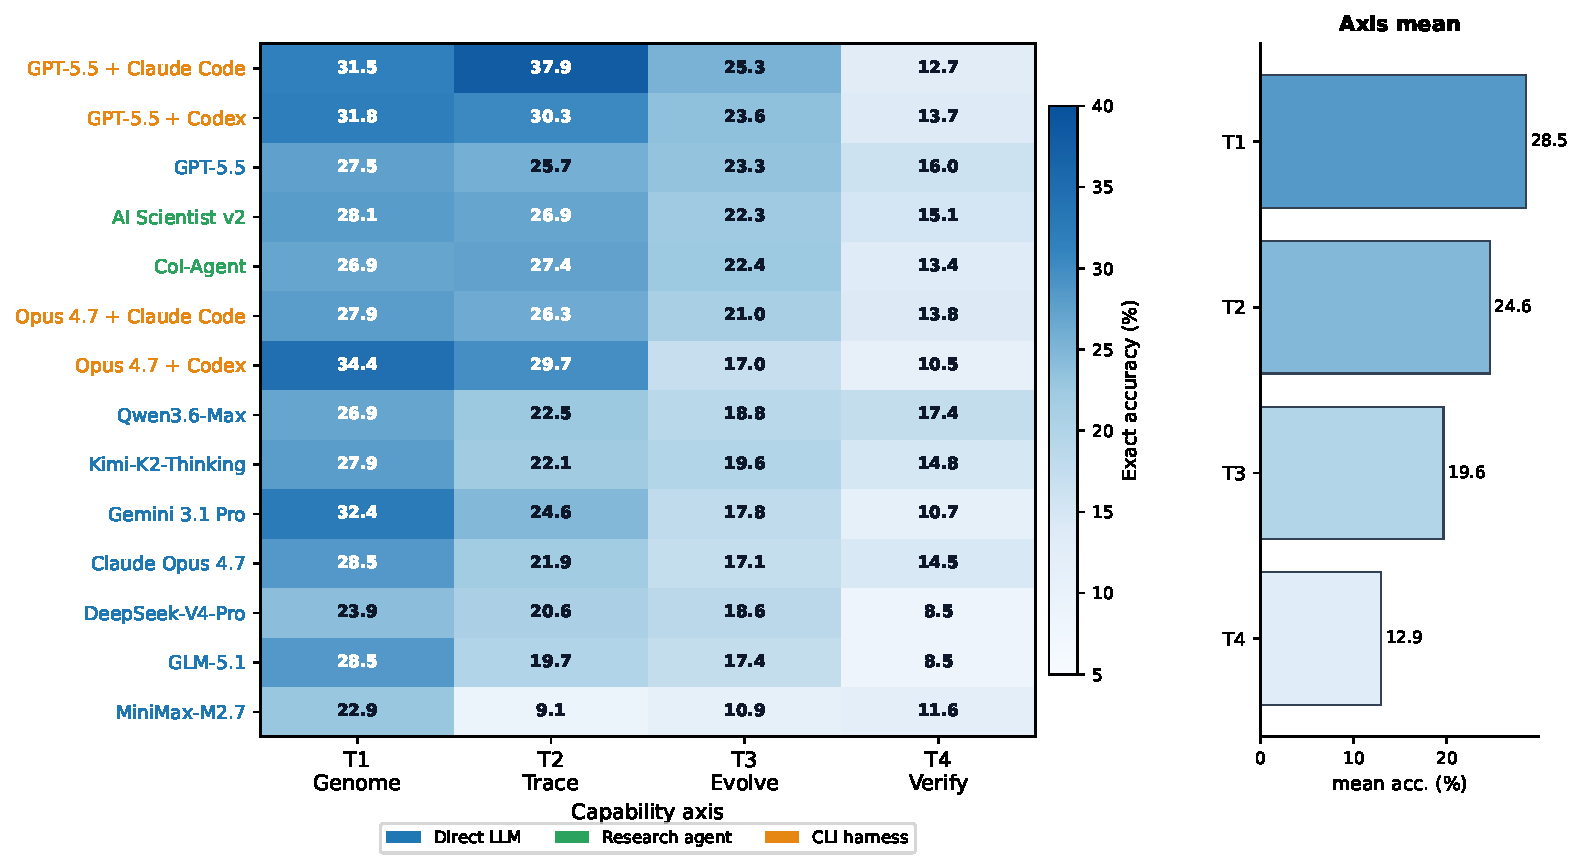
\includegraphics[width=0.72\textwidth]{figures/exam_bottleneck.pdf}
\caption{\textbf{\geneexam{} exact-accuracy heatmap.} Exact accuracy across T1--T4 for all evaluated systems, with verification remaining the hardest axis.}
\label{fig:exam_bottleneck_app}
\end{figure}

\subsection{Error Analysis: Failure Flow}

This Sankey view aggregates wrong answers by capability tier, failed field family, and error class. It is meant to localize the bottleneck: most failures originate in evolutionary reasoning and verification, then propagate through driver and dynamics fields before becoming exact-match errors.

\begin{figure}[h]
\centering
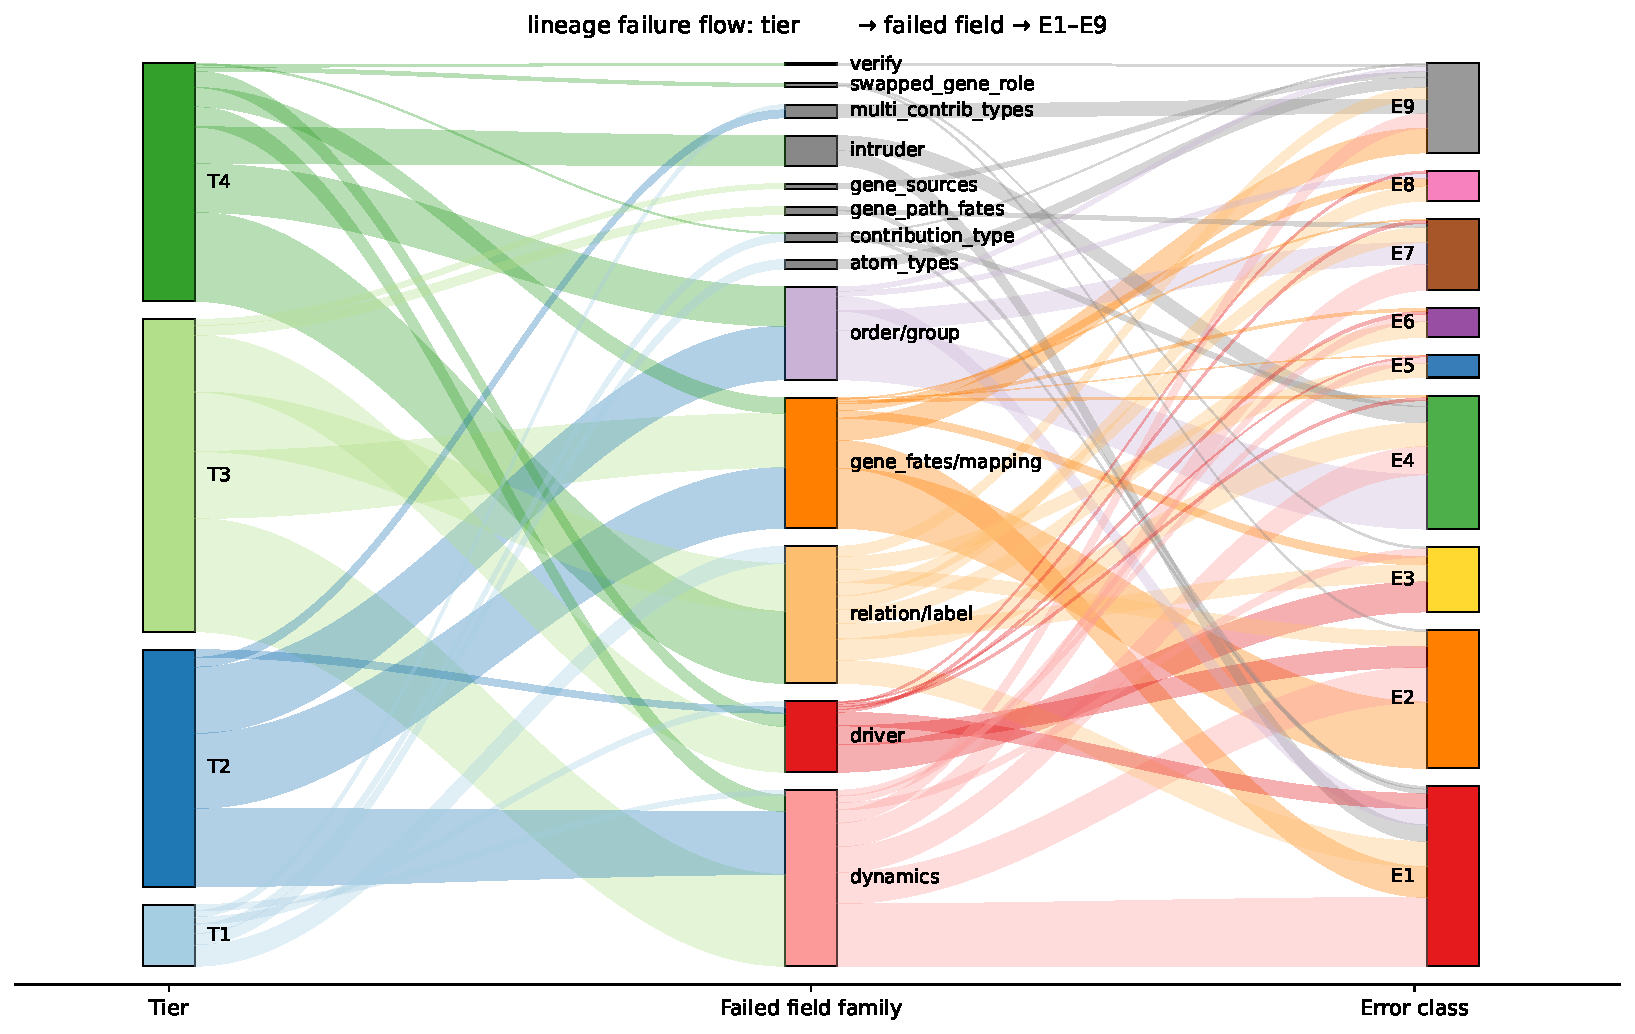
\includegraphics[width=0.85\textwidth]{figures/error_sankey.pdf}
\caption{\textbf{\geneexam{} failure flow.} Sankey diagram tracing errors from capability tier (T1--T4) through failed field family to error class (E1--E9). T3 and T4 errors dominate in volume. The thickest flows connect T3/T4 to dynamics and driver fields, which then fan out to E1 (dynamics misclassification) and E2 (driver misidentification). Genome-fate and relation errors (E3--E4) are the next largest classes, confirming that compositional field interactions---not isolated label failures---drive the accuracy bottleneck.}
\label{fig:error_sankey_app}
\end{figure}
